\section{Uncertainty Quantification} \label{uq}
\thispagestyle{plain} % surpress header on first page

Most sciences work at least to a certain degree quantitatively and by doing so they often rely on theoretical models that in many cases approximate the underlying true mechanisms that drive a certain process or phenomenon. In many cases the quantitative model outcome of interest is the result of a transformation of model inputs through a complex mathematical system. Across disciplines, from a model perspective many inputs and initial states as well as their development are not deterministic but are uncertain. The model inputs are often informed by theory, previous quantitative studies as well as experiments or need to be calibrated using limited data but cannot be treated as known. It is now often argued that the inherently uncertain parameters propagate their error through the model which yields an uncertain model outcome. In order to make informed decisions based on the model outcome, this uncertainty should be quantified and communicated. This constitutes one main motivation why the applied mathematics field of Uncertainty Quantification (UQ) developed and still is an active field of research. Many of its advancements come from the engineering and physical sciences in which negligence of uncertainty in the outcomes can lead to attributable and severe consequences. In climatology, the predicted path of a hurricane is reported with uncertainties which are due to the dynamical, complex weather conditions that can only be approximated. These uncertainties inform countries about whether they might be hit while giving them valuable time to prepare. An example from engineering involves the safety of a nuclear power plant which in turn is affected by factors such as the weather and its environment in general. This also includes seismological activity which was causing the catastrophe in Fukushima back in 2011. Uncertainty Quantification tries to incorporate those risks in the modeling process and make them explicit (compare \cite{Sullivan.2015} and \cite{Smith.2013}).

Taking a step back from those very precise motivations for UQ, \cite{Smith.2019} make a simple mathematical point suggesting that it is worth to investigate uncertainty. Their motivation rests on the butterfly effect (see \cite{Lorenz.1963}) which demonstrates that already a slight perturbation in initial conditions can result in an unforeseeable change in the outcome of a complex dynamical system over time. Going back to our initial observation that models often are complex mathematical systems, this provokes the thought that also in this case small changes in inputs might have a strong impact on model predictions. But how does that matter in Economics? And how do we quantify this uncertainty? An answer to the first question and a motivation for UQ can be found in a recent study by \cite{Cai.2019}. They estimate "the social cost of carbon (SCC), defined as the marginal economic loss caused by an extra metric ton of atmospheric carbon" \footnote{ Compare page 3 in \cite{Cai.2019}.} based on the Dynamic Integrated Climate–Economy” (DICE) model (\cite{Nordhaus.1992, Nordhaus.2008}). They add uncertainty regarding the economic development as well as the change in climate conditions to this framework by assuming possible ranges of those factors and propagate them through their model. The result is quite astonishing as for the year 2005 the SCC varies between 59 to 99 Dollars per ton of carbon for a realistic range of projections in economic and climatic outlook. This range of uncertainty in the model outcome is quite large but clearly sends a more informative message to policy makers.

While it is well understood in Economics that there is uncertainty affecting model outcomes and hence policy recommendations as well as that its communication is crucial, it is rarely the case that a full, coherent evaluation of uncertainties is performed that goes beyond robustness checks (see \cite{Manski.2019} and \cite{Scheidegger.2019}). This is where the already existent UQ framework can come in and answer the second question from before, how to quantify uncertainty and determine which sources are contributing to it as recently done in \cite{Scheidegger.2019} and in \cite{Harenberg.2019}. In the following, I will introduce the cornerstones of this framework and apply some of its general ideas to the Rust model and the comparison of MPEC and the NFXP.

\subsection{The UQ Framework}

For the following description I mainly rely on \cite{Smith.2013} who outlines a comprehensive UQ framework with a focus on engineering and physics as well as on \cite{Oberkampf.2010} who deal with uncertainty in a more general scientific computing context.  The starting point for both is the observation that there are many potential sources of uncertainty that can affect the outcome of a computational model. First, there is model uncertainty which translates into the underlying mathematical framework of a model. In many cases the true underlying process that the mathematical model is supposed to capture is not perfectly understood which renders the mathematical representation imprecise. In the Rust Model we impose the behavioral assumption on Harold Zurcher that his decision process follows that of a maximization of his discounted life time utility over an infinite horizon. We do not know whether this is warranted and even if it was, on a lower level there is still uncertainty about how his underlying cost function exactly looks like for example. Quite obviously the choice of the specific mathematical representation affects the predictions the model will make after being calibrated. A second source are the parameter inputs themselves. As in Economics they usually are estimated from data, there always remains uncertainty around the specific parameter estimates. This parameter uncertainty translates into uncertainty of the model outcomes. Thirdly, in many applications the computational implementation of a mathematical model involves approximate numerical solutions to the whole model itself or at least parts of it. In our example, we rely on numerical optimization algorithms that introduce some error but also the discretizing of the expected value function is solely an approximation of the true mathematical relation. A last factor is a potential measurement error in the model inputs. This could be for instance an imprecise measurement of the cumulative mileage state of some buses.

The authors argue now that the very nature of those uncertainties can be different. On the one hand, the uncertainty can be \textit{aleatoric} which means that it is stochastic and cannot be reduced by gaining additional economic or experimental knowledge. For those uncertainties there typically exists a probability distribution. On the other hand, there is \textit{epistemic} uncertainty which can generally be reduced. It includes for example the previously stated uncertainty of the correct cost function which might be solved by running an experiment. For this example, there clearly is no probability distribution describing the error but rather an interval of different possible uncertainties. Given that some of these uncertainties are uncovered in a specific model, the UQ framework prescribes the following two steps. However, before we dive into this, let us first refine the terms of model and model outcome. In the UQ framework, the computational model can be described like this:

\begin{equation}
	y = f(\theta)
	\label{compmodel}
\end{equation}

where $\theta$ are the model inputs or parameters and $y \in \mathbb{R}^Q$ the model output or the quantity of interest (QoI). \paragraph{}
The QoI can be any policy relevant vector or scalar that could be obtained from the underlying mathematical model. In \cite{Cai.2019} this is the social cost of carbon. In my thesis, this will be some counterfactual demand level for bus engines given a certain replacement cost. I will further go into detail about this in the next section. This computational model itself can already suffer from discrepancies to the true mathematical model due to model errors and numerical errors. Given that the model parameters have to be calibrated from data and hence suffer from uncertainty in the estimates, they are represented by a random vector $\Theta$ which has a certain probability distribution depending on the data at hand. Given the calibrated parameters, the uncertainty in the parameters affect the model outcome in the following way:

\begin{equation}
	Y = f(\Theta)
	\label{uncertaincompmodel}
\end{equation}

with $Y$ being the QoI that itself is a random vector or variable. \paragraph{}

The fact that measurement, numerical and model uncertainty might exist is implicitly included in the fact that the computational model $f(.)$ is not equivalent to the true mathematical model, i.e. the QoI $y$ and the parameter vector $\theta$ are already not deterministic but rather uncertain affected by the above mentioned errors.

Coming back to our two steps in the UQ framework, first, the uncertainties are accounted for in the model inputs and then propagated through the model. Second, this propagation is then accounted for in some uncertainty around the quantity of interest. In a sub field of UQ, \textit{sensitivity analysis}, this propagation technique is exploited to determine which parameters of the model contribute the most to the observed uncertainty in the QoI. This can be of great interest even beyond the argument of informed policy decisions as it can give valuable information to researchers that want to calibrate a certain economic model with actual data. It gives them an indication which parameters to focus on during the calibration procedure which in turn might reduce the uncertainty in the QoI. This analysis further conveys information about the mathematical model itself an how it could be refined to provoke a lower uncertainty around the QoI (see \cite{Scheidegger.2019},  \cite{Harenberg.2019} and \cite{Ghanem.2017}). In this literature, usually a host of combinations of different parametrizations are used to propagate through the model and calculate its QoI. This information from several runs is then used to systematically determine the influence of the uncertainty in specific parameters on the uncertainty in the QoI. With increasing complexity of the computational model, this becomes computationally infeasible as it would involve too many runs of the model. This is the reason why the literature developed so called surrogate models that approximate the true computational model while maintaining higher speed of convergence for a single run (compare also \cite{Saltelli.2008}). While this strand of literature focuses on parameter uncertainty, in the setting of economic models it also implicitly takes some other forms of uncertainty from the calibration procedure into account as the exact estimate of a parameter depends also on model and numerical specifications in the calibration procedure. In many cases, though, a potential model or numerical error will also affect the QoI directly and not solely through the parameter uncertainty as will be the case in what is about to follow.

First, though, in the following section I will introduce the mathematical and computational model for the QoI from which the remainder of my thesis will draw.

\subsection{The Quantity of Interest: The Demand Function}

\cite{Rust.1987} shortly describes a way to uncover an implied demand function of engine replacement from his model in combination with estimated parameters. Theoretically, for Harold Zurcher the random annual implied demand function takes the following form:

\begin{equation*}
	\tilde{d}(RC) = \sum_{t=1}^{12} \sum_{m=1}^{M} \tilde{d}^m_t
\end{equation*}

while $\tilde{d}^m_t$ is the replacement decision for a certain bus $m$ in a certain month $t$ derived from the process \{$d^m_t$, $x^m_t$\}. For convenience I will drop the index for the bus in the following. Its probability distribution is therefore the result of the process described by $P(d_t|x_t; \theta)p_3(x_t|x_{t-1}, d_{t-1}; \theta_3)$. For simplification \citeauthor{Rust.1987} actually derives the expected demand function $d(RC)=\E[\tilde{d}(RC)]$. Assuming that $\pi$ is the long-run stationary distribution of the process \{$d_t$, $x_t$\} and that the observed initial state \{$x_0$, $d_0$\} is in the long run equilibrium, $\pi$ can be described by the following functional equation:

\begin{equation}
	\label{eq18}
	\pi(x, d; \theta) = \int_{y} \int_{j} P(d|x; \theta)p_3(x|y, j; \theta_3) \pi(dy, dj; \theta).
\end{equation}

Further assuming that the processes of \{$d_t$, $x_t$\} are independent across buses the annual expected implied demand function boils down to:

\begin{equation}
	\label{eq19}
	d(RC) = 12 M \int_{0}^{\infty} \pi(dx, 1; \theta).
\end{equation}

Given some estimated parameters $\hat\theta$ from calibrating the Rust Model and parametrically varying $RC$ results in different estimates of $P(d_t|x_t; \theta)p_3(x_t|x_{t-1}, d_{t-1}; \theta_3)$ which in turn affects the probability distribution $\pi$ which changes the implied demand. In the representation above it is clearly assumed that both the mileage state $x$ and the replacement decision $d$ are continuous. The replacement decision is actually discrete, though, and the mileage state has to be discretized again which in the end results in a sum representation of equation \ref{eq18} that is taken to calculate the expected annual demand function.
\paragraph{}

A flexible calculation of the above demand function depending on some parameter vector $\theta$ has been implemented by me in the ruspy package which I will rely on in the following. I will now showcase the UQ framework for uncertainty propagation by using the resulting empirical distribution function of the parameter vector $\hat\theta$ from the Monte Carlo simulation in \ref{generalsetup}, propagate it through the model (the calculation of the demand function) and obtain the distribution of a QoI (a certain demand level for a given $RC$) and consequently the uncertainty in its estimate.

\subsection{Uncertainty Propagation of the Simulation in Iskhakov et al. (2016)}

For this section I draw on the results of the Monte Carlo simulation for the discount factor $\beta=0.975$ from section \ref{generalsetup}. As the results for MPEC and NFXP are virtually the same and they do not vary across different starting values, I rely on the MPEC results for the starting values $(RC^0, \theta^0_{11}) = (4,1)$.

\begin{figure}[!t]
	\caption{Joint Distribution of $\hat{RC}$ and $\hat\theta_{11}$}
	\centering
	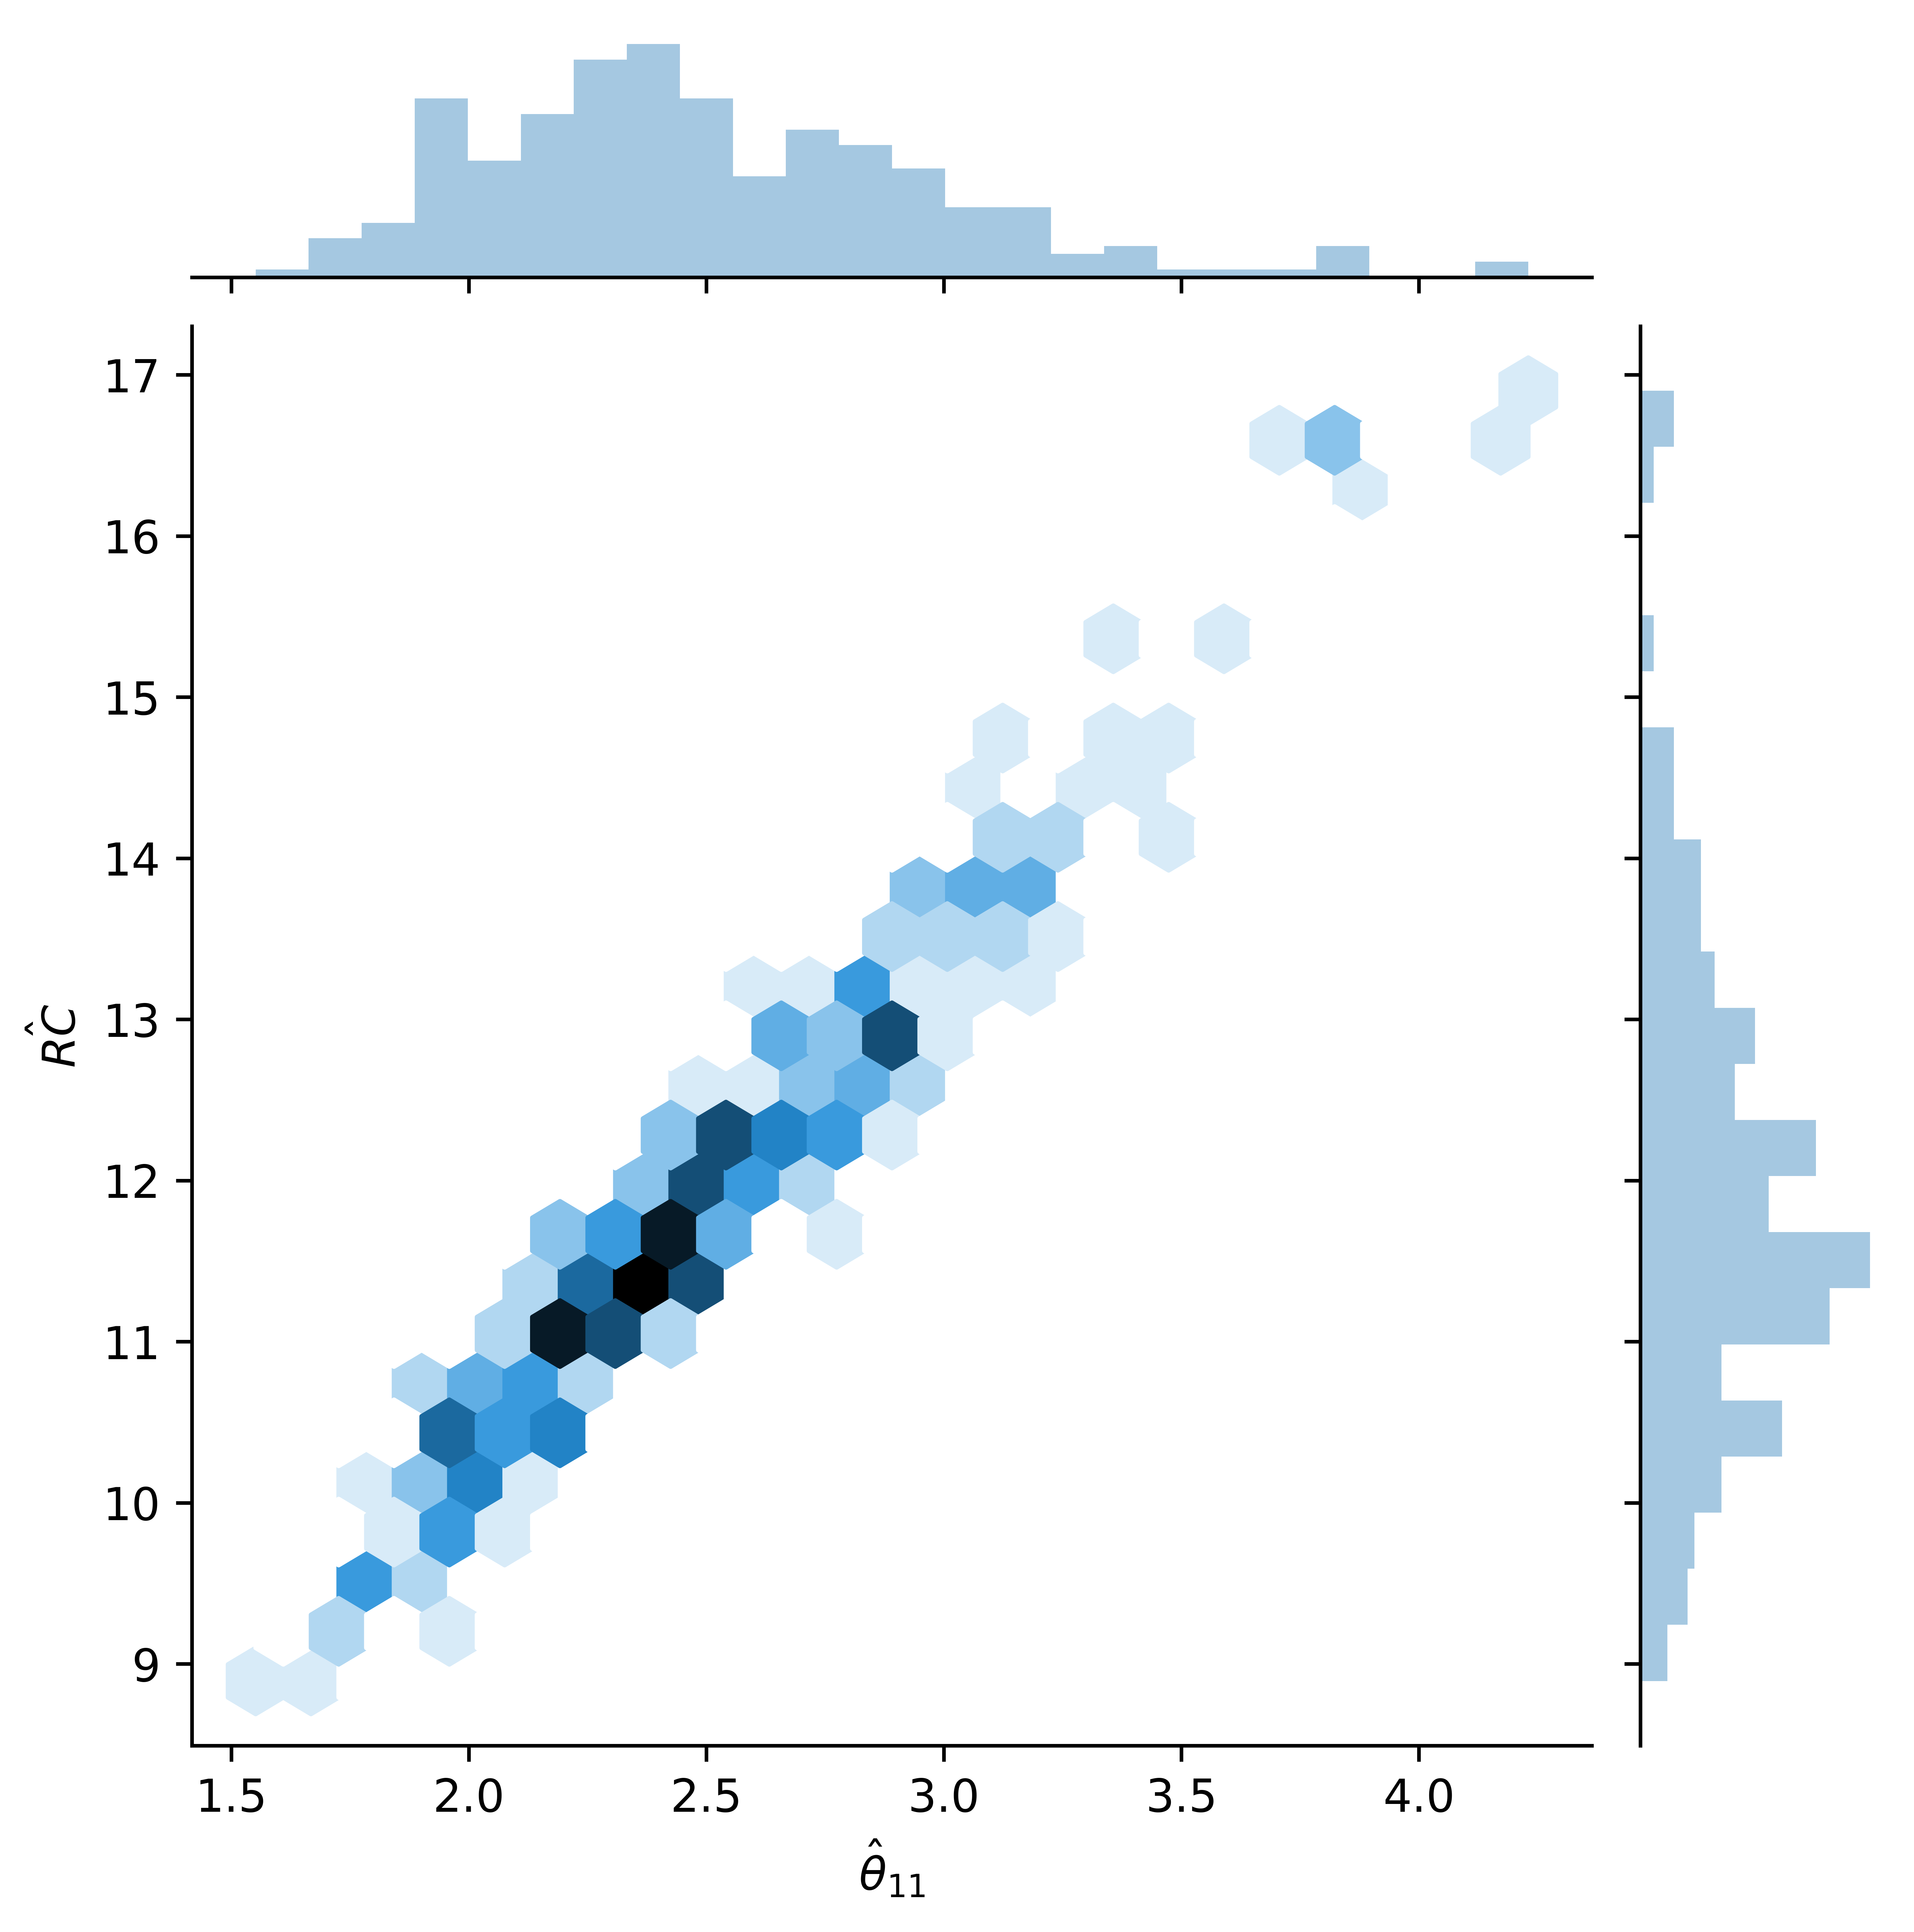
\includegraphics[scale=0.8]{../figures/figure_2.png}
	\label{figure2}
\end{figure}

Hence, in total I have 250 parameter estimates for 250 different data sets that were, as \cite{Su.Judd.2012} point out, created by a parametric bootstrap procedure. This allows me to identify summary statistics for both the parameters as well as the QoI. As we keep both the model assumptions and numerical approximations constant across the runs, we solely have a look at the effect of uncertainty in the parameters from the calibration process on the QoI. In the context of \textit{sensitivity analysis} which is targeting the influence of parameter uncertainty it is important to first determine whether the uncertainty in parameters is actually independent across them or whether there is some interdependence as it determines which techniques can actually give reliable results (\cite{Saltelli.2008}). The correlation between all parameters is reported in Table \ref{table2} in appendix A. Here, I visualize the joint distribution of the cost parameter estimates in Figure \ref{figure2} which shows that there is a strong interdependence between them. Consequently, an approach to sensitivity analysis in which only one parameter at a time is varied to determine its contribution to the uncertainty in the QoI would lead to wrong results. In the above Figure \ref{figure2} we can further observe that the empirical distribution of our estimates is centered around the true values of the cost parameters and that the actual overestimation of them (compare to section \ref{appendixC} in the appendix) seems to be driven by some outliers that yield estimates being way too large.

\begin{figure}[!t]
	\caption{Distribution of the QoI}
	\vspace*{-4mm}
	\centering
	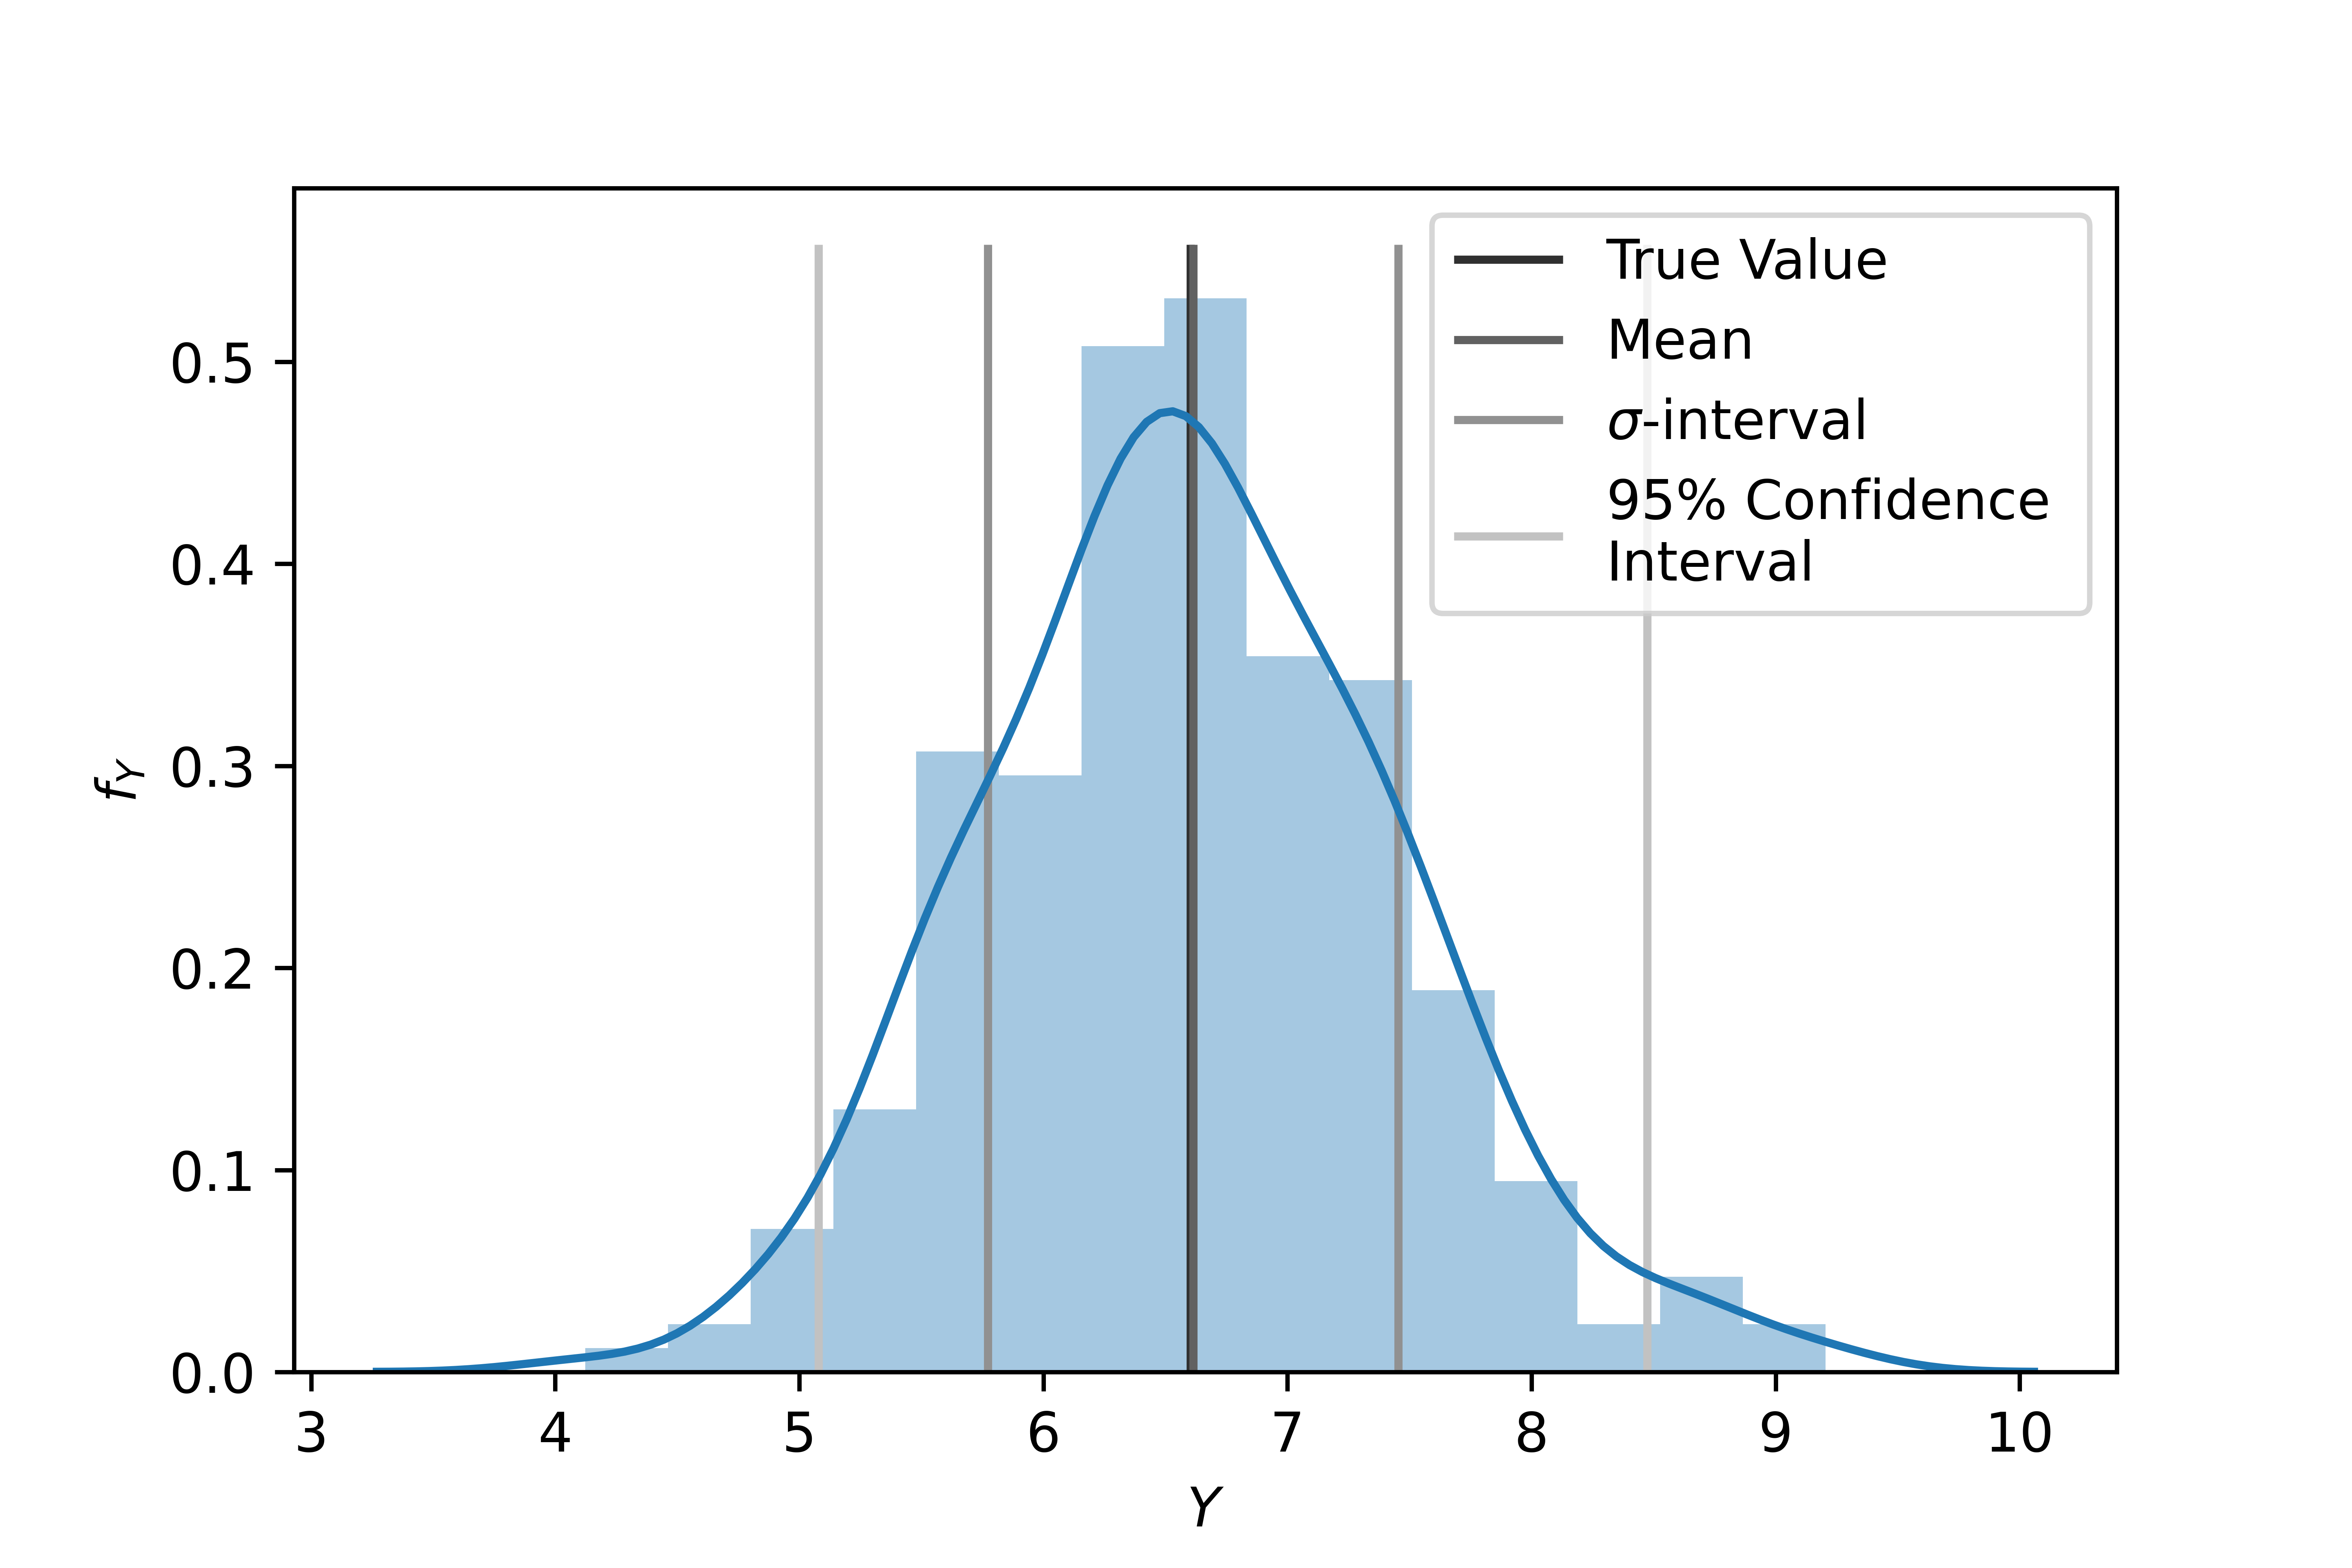
\includegraphics[scale=0.9]{../figures/figure_3.png}
	\label{figure3}
\end{figure}

We are now interested in how this parameter uncertainty translates into uncertainty around some quantity of interest. For the remainder of this paper I am interested in how high expected annual demand for bus engines will be if the equilibrium price for engine replacement drops to 11,000 Dollars (as a reminder the cost function is scaled by 0.001 which means that the true $RC$ corresponds to 11,725.70 Dollars) and the bus fleet consists of 50 buses. In the language of the UQ framework the demand function in equation \ref{eq19} corresponds to the computation model $f(.)$ in equation \ref{compmodel} and \ref{uncertaincompmodel}. The propagation of the random vector $\Theta = (\hat{RC}, \hat\theta_{11}, \hat\theta_3)^{N=250}_n$ across the Monte Carlo runs results in the random vector $Y$ which equals to the expected annual demand at replacement costs of 11,000 Dollars. The uncertainty in the QoI $Y$ is depicted in Figure \ref{figure3}.


The calculated empirical mean of $Y$ across the Monte Carlo runs is very similar to the true expected demand (which is derived from the true parameter vector). The interval of one standard deviation around the mean ranges from around 5.8 to 7.5 while the 95\% bootstrap confidence interval stretches from 5.1 to 8.5.\footnote{The percentile bootstrap is used (compare \cite{Davison.1997} chapter 5).} This uncertainty obviously also translates into the view on the whole expected demand function across a range of different replacement costs. Figure \ref{figure4} below corresponds to the implied demand function in Figure 7 of \cite{Rust.1987} while being calculated for 50 buses and for the model setup of \cite{Iskhakov.2016}. To Rust's figure I now add uncertainty resulting from the calibration procedure. I obtain a well-behaved downward sloping demand function for which the mean across our Monte Carlo simulation corresponds closely to the true expected demand function.

This constitutes the end of the description on the basic idea of uncertainty quantification in the Rust Model. In the next sections, I will use this framework to vary other key specifications of the model and the calibration procedure to investigate how this translates into the uncertainty of the QoI described above and whether this might differ when using MPEC as opposed to the NFXP.

\begin{figure}[H]
	\caption{The Implied Demand Function accounting for Parameter Uncertainty}
	\vspace*{-4mm}
	\centering
	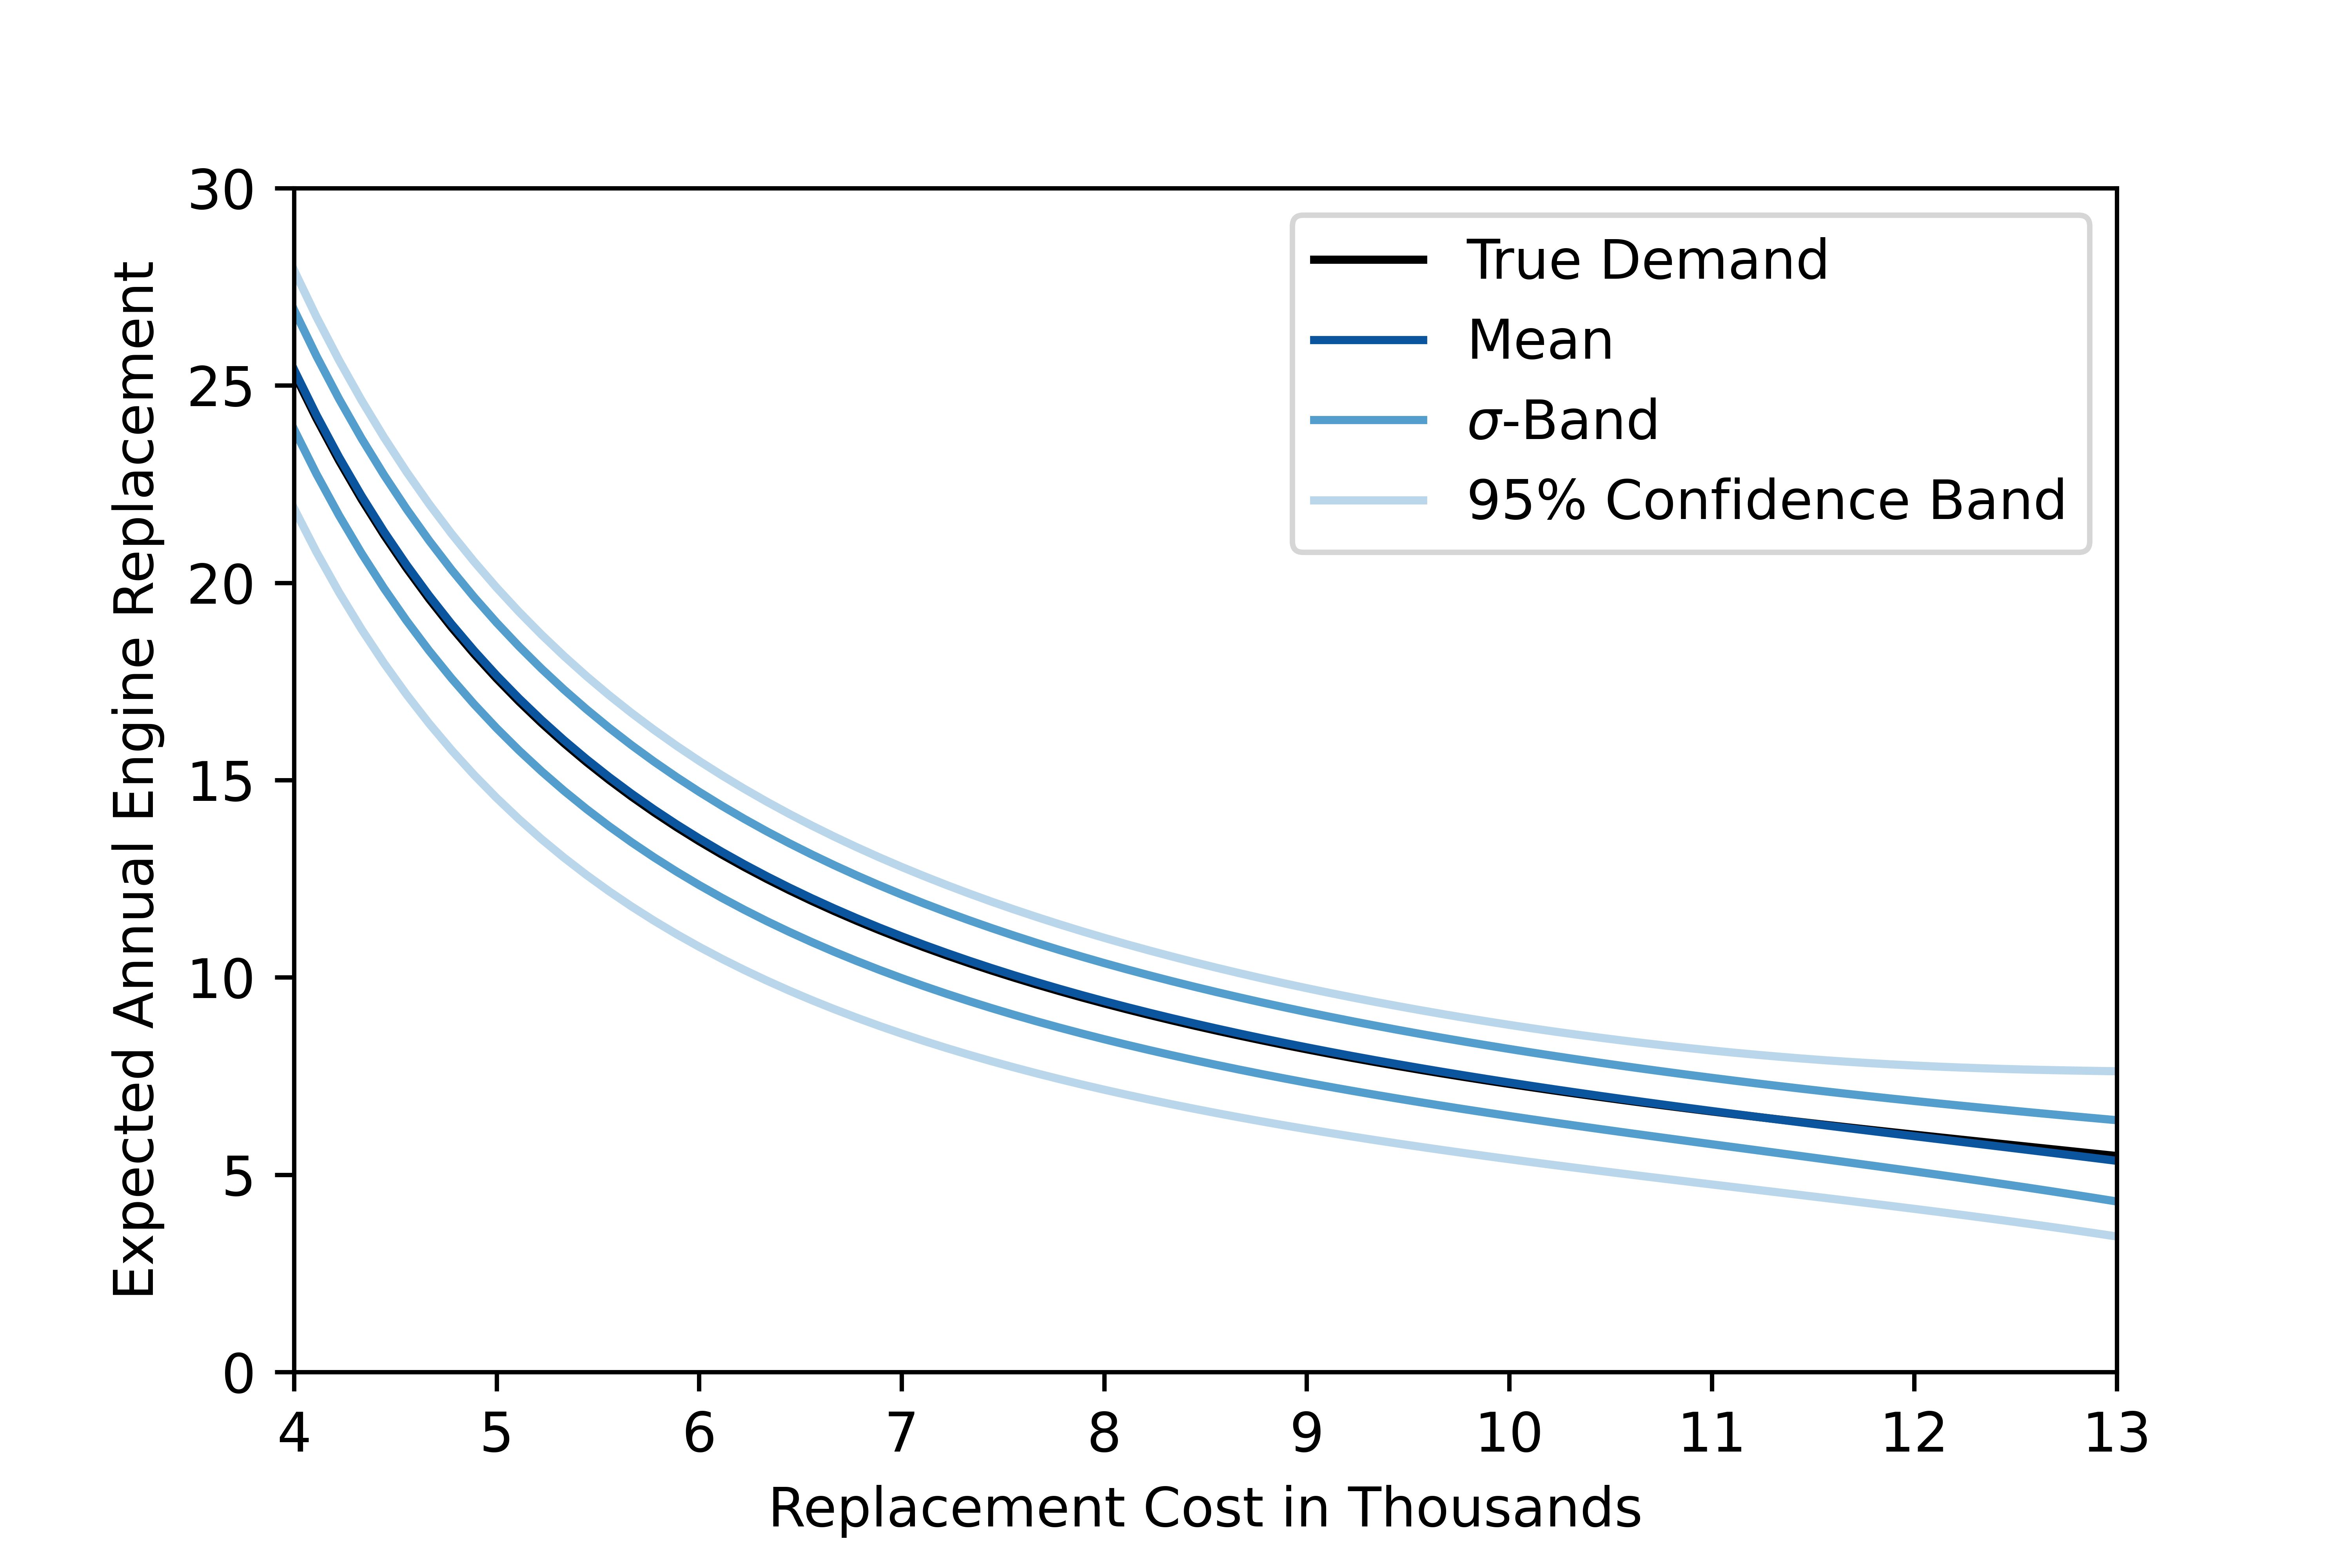
\includegraphics[scale=0.9]{../figures/figure_4.png}
	\label{figure4}
\end{figure}








